\section{What is Statistical Inference?}

\begin{frame}
  \begin{center}
    {\bf Part I -- What is Statistical Inference?}
  \end{center}
\end{frame}

\subsection{Introduction}
\begin{frame}{Summary and Outline}
  \begin{itemize}
    \item In the last lecture, we talked about {\bf descriptive statistics}:
    \begin{itemize}
      \item Describe the system we want to study using experiment data and statistics;
      \item Point Estimators: Calculate a specific value (parameter) of the population;
      \item Interval Estimator: Shows the error/confidence of our estimation;
    \end{itemize}\bigskip

    \item In some cases, a description alone is not enough.
    \item We want to make an "informed decision" about the data.
    \begin{itemize}
      \item "Given some experimental data, can I conclude {\bf X}?"

    \end{itemize}\bigskip

    \item {\bf Statistical Inference} is tool for making decisions/conclusions from data.
  \end{itemize}
\end{frame}

\begin{frame}{Example of when we need Statistical Inference}
  \begin{columns}
    \column{.8\textwidth}
    You are the owner of a factory that produces delicious chocolate.\bigskip

    The packages that you produce and sell should contain \structure{around 300g of chocolate}. (Of course there is some variation) \bigskip

    Every 6 months, you want to check if your production line is working correctly. If not, you need to schedule \emph{maintenance}.\bigskip

    How do you check if your factory needs maintenance or not?
    \column{.2\textwidth}
    \hfill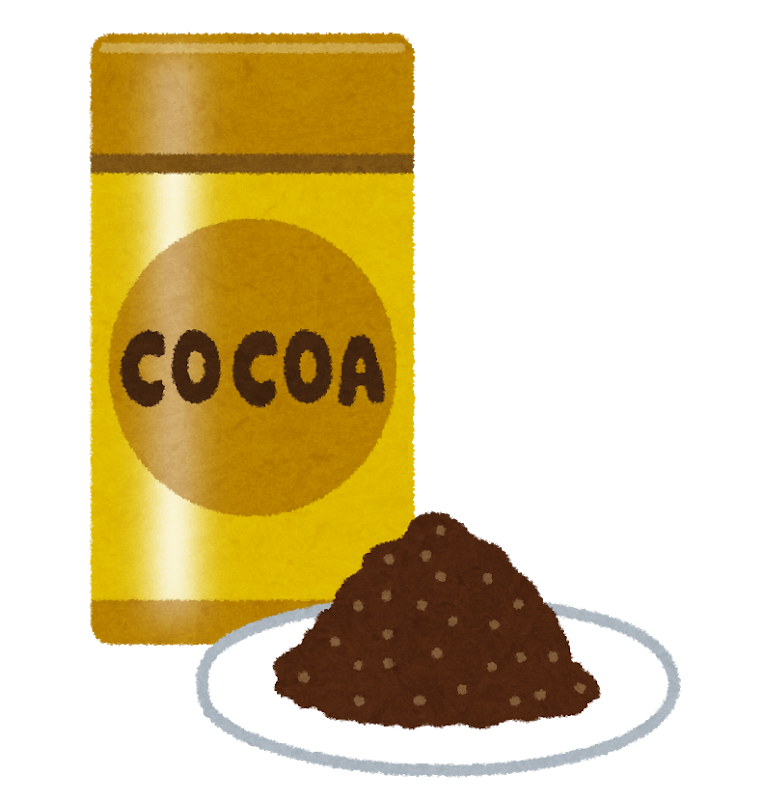
\includegraphics[width=1\textwidth]{../img/irasutoya_cocoa}
    \ppagenote{Cocoa image from \url{https://www.irasutoya.com}}
  \end{columns}\bigskip
\end{frame}

\begin{frame}{Example of when we need Statistical Inference}
  \begin{columns}[T]
    \column{.8\textwidth}
    Using the knowledge of this class, you make an experiment.\\
    You take a sample of {\bf 30 packages} from the facture and weight them.\bigskip

    First, you calculate the sample's average weight: {\bf 295g}\bigskip

    Then you remember last lecture, and calculate the\\
    95\% confidence interval: {\bf 283g to 307g}.\bigskip
    \column{.2\textwidth}
    \hfill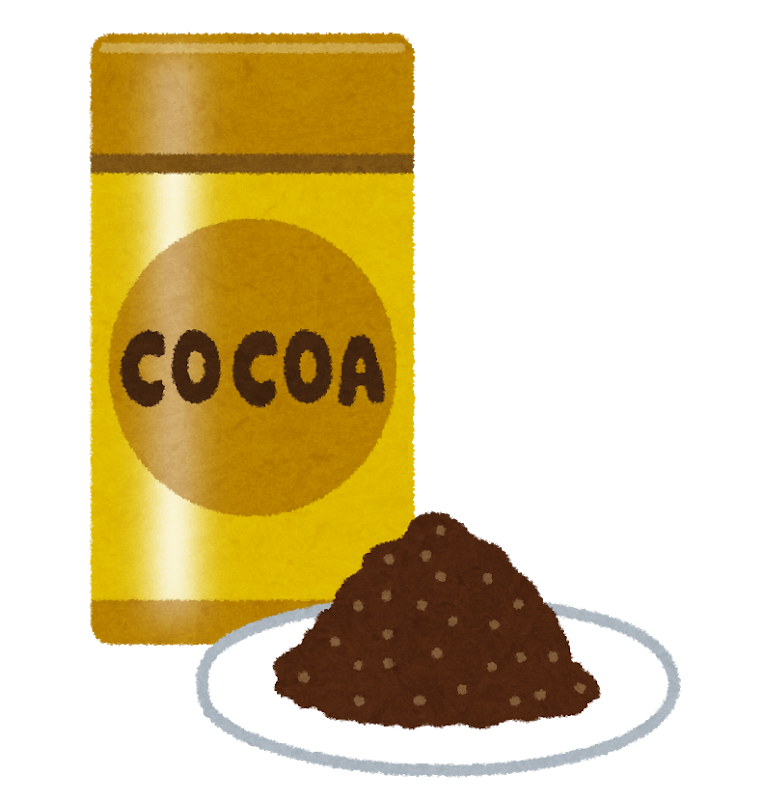
\includegraphics[width=1\textwidth]{../img/irasutoya_cocoa}
    \ppagenote{Cocoa image from \url{https://www.irasutoya.com}}
  \end{columns}\bigskip

  From this data, do you believe that the mean production of your factory is 300g? Or is it necessary to investigate further?\bigskip

  You need more information to make that decision!
\end{frame}

\subsection{Definitions}

\begin{frame}{Enter Statistical Inference:}
  \begin{block}{}
    {\bf Statistical inference} is a process that uses data analysis to establish the (probable) truth of a statement. (compare with logical inference)
  \end{block}\bigskip
  \begin{columns}[T]
    \column{.25\textwidth}
      \includegraphics[width=\textwidth]{../img/sampling_distribution}
    \column{.7\textwidth}
%      Remember a few facts:
      \begin{itemize}
        \item We create a \structure{probabilistic model} that describes our system of interest, and the possible outcomes of an experiment.
        \item The statistics calculated from \structure{sample data} can be described as random variables, and analized.
      \end{itemize}\bigskip

      Using the sample data, we can compare the characteristics of the sample (sample model) with the assumed characteristics of the population (population model).
  \end{columns}\bigskip

  \begin{center}
  Sample data $\rightarrow$ parameter estimation $\rightarrow$ compare with model $\rightarrow$ statistical inference
  \end{center}
\end{frame}

\begin{frame}{Statistical Hypothesis}
  \structure{(Statistical) Hypothesis} is a key concept of statistical inference.
  \begin{itemize}
    \item {\bf Hypothesis:} a statement that explains a phenomenom we observe;
    \item {\bf Statistical Hypothesis:} an statement about a {\bf statistical} model;
  \end{itemize}\bigskip

  \begin{columns}[T]
    \column{0.8\textwidth}
    \structure{Back to our example.} We want to know if our chocolate factory is working normally. Our packages should have, on average, at least 300g of chocolate (or we might get sued!).

    \begin{block}{Statistical Hypothesis}
    The \structure{population model} that describes the weight of a package in our factory has a {\bf mean} of at least 300g. $(\mu_{\text{weight}} \ge 300)$
    \end{block}


    \column{0.2\textwidth}
    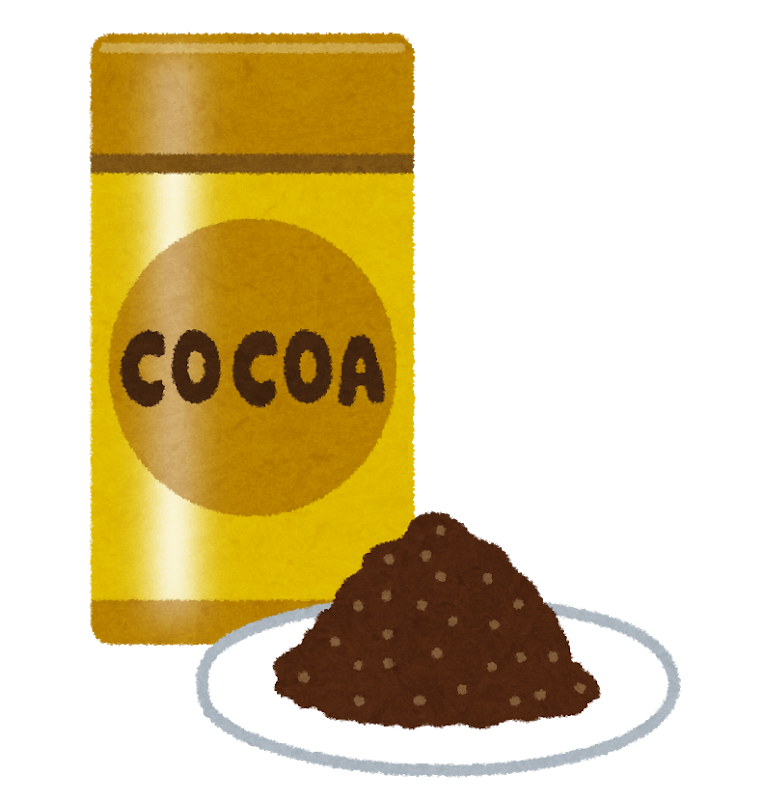
\includegraphics[width=\textwidth]{../img/irasutoya_cocoa}
  \end{columns}
  \vfill
  \alert{Pay attention!} Note how the \emph{scientific question} leads to the \emph{statistical hypothesis}.
\end{frame}

\subsection{All about Hypothesis}
\begin{frame}{Statistical Hypothesis}{Common Hypotheses and Statistical Hypotheses}
  \begin{itemize}
    \item {\bf Common Hypothesis:} a general statement about what we believe about the world;
    \item {\bf Statistical Hypothesis:} an statement about parameters in a {\bf statistical} model;
  \end{itemize}\bigskip

  {\smaller
  \alert{Common Hypothesis:} The factory is broken, and producing less cocoa than normal.\\
  \structure{Statistical Hypothesis:} The mean weight of packages produced is less than 300g\\
  \medskip

  \alert{Common Hypothesis:} The proposed algorithm is faster than standard algorithms.\\
  \structure{Statistical Hypothesis:} The difference in mean execution time between the proposed and the standard algorithm is above 2s\\
  \medskip

  \alert{Common Hypothesis:} Cats are more popular than dogs.\\
  \structure{Statistical Hypothesis:} The proportion of cat videos on Youtube that are watched until the end is 5\% higher than the proportion of dog videos watched until the end.
  }

  \vfill

  One easy way to think about it, is that a statistical hypothesis can always be represented as an equation.
\end{frame}

\begin{frame}{Statistical Hypothesis}{What is a good hypothesis?}

  Here are some characteristics of a useful {\bf scientific hypothesis} (statistical or not).\\
  Keep these characteristics in mind when you create your hypotheses:\bigskip

  \begin{itemize}
    \item {\bf Predictive power}: The hypothesis not only explains the existing data, it helps you predict future data.
    \begin{itemize}
      \item There were mistakes in the production because the workers were tired yesterday.
      \item There were mistakes in the production because the workers are tired on Mondays.
    \end{itemize}

    \item {\bf Principle of parsimony} (Ockam's razor): The hypothesis makes few assumptions about the system:
    \begin{itemize}
      \item Energy usage pattern is described by this neural network with 1.000.000 parameters.
      \item Energy usage pattern is described by this 3rd degree polynomial.
    \end{itemize}

    \item {\bf External consistency}: The hypothesis fits with existing, well accepted knowledge about the system.
    \begin{itemize}
      \item Mean global temperature is correlated with the number of active pirates;
      \item Mean global temperature is correlated with CO2 emmissions;
    \end{itemize}
  \end{itemize}
\end{frame}

\begin{frame}{Hypothesis and Experiments}{How do we use hypotheses?}
  General approach:
  \begin{itemize}
    \item Create multiple hypothesis for the phenomenom that we are studying.
    \item Run experiment and decide which hypothesis fits the data best.
  \end{itemize}\bigskip

  {\bf 1. Create Hypotheses:}
  \begin{itemize}
    \item H1: The mean weight of packages produced by the factory is above 300g.
    \item H2: The factory is broken and producing packages with much less than 300g.
  \end{itemize}\bigskip

  {\bf 2. Obtain Data: Collect 10 cocoa packages randomly, and weight them}
  \begin{itemize}
    \item Weights: 293 325 \alert{271} 313 309 298 284 304 \alert{248} 296
    \item Sample average: 294g\\
    \item Minimum and maximum: 248g, 325g\\
  \end{itemize}
\end{frame}



\begin{frame}{Hypothesis, Experiments, and Statistical Inference}
  The \structure{statistical inference} process helps us choose which hypothesis fits the experimental data best. Given the sample data $x$, we calculate the {\bf probability that $x$ is observed if the hypothesis $H_i$ is true}: $P(x|H_1), P(x|H_2), P(x|H_3), \ldots$
  \bigskip

  We give more credibility for the hypothesis that maximizes the probability of the data.\bigskip

  {\bf Example:} $x = \{293, 325, 271, 313, 309, 298, 284, 304, 248, 296\}$

  \begin{columns}
    \column{0.4\textwidth}
    \begin{block}{Hypothesis 1: $\mu \geq 300$}
      What is the probability that we see the sample $x$ when the mean production of the factory is 300g or more?
    \end{block}
    \column{0.2\textwidth}
    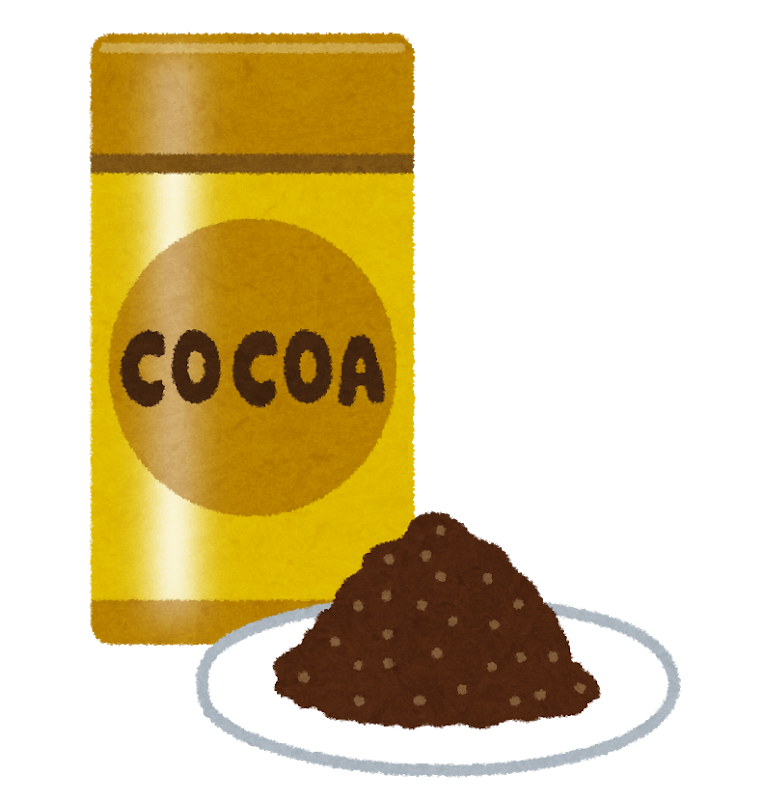
\includegraphics[width=\textwidth]{../img/irasutoya_cocoa}
    \column{0.4\textwidth}
    \begin{block}{Hypothesis 2: $\mu < 300 - \delta$}
      What is the probability that we see the sample $x$ when the mean production of the factory is $\delta$ less than 300g?
    \end{block}
  \end{columns}
\end{frame}

\subsection{Null Hypothesis Testing}
\begin{frame}{Null Hypothesis Significance Testing (NHST)}
  The NHST approach for statistical inference involves the contrast between\\
  a {\bf null hypothesis} and an {\bf alternate hypothesis}.\bigskip

  \begin{columns}[T]
    \column{0.5\textwidth}
    \structure{Null Hypothesis ($H_0$)}
      \begin{itemize}
        \item Absence of effects;
        \item Conservative model;
        \item "nothing special is happening"
      \end{itemize}
      \bigskip

      "As expected, the mean weight packages produced in the factory is at least 300g"
      \bigskip

      {\bf $H_0: \mu \geq 300$}
    \column{0.5\textwidth}
    \structure{Alternative Hypothesis ($H_1$)}
      \begin{itemize}
        \item Presence of some effect;
        \item Something "new" is happening;
      \end{itemize}
      \bigskip

      "There is \alert{an anomaly} in the factory, and the mean production is below 300g"
      \bigskip

      {\bf $H_1: \mu < 300$}
  \end{columns}
\end{frame}

\begin{frame}{Null Hypothesis Significance Testing (NHST)}{How to choose a null hypothesis?}
  \begin{itemize}
    \item Use existing knowledge about the process being investigated;
    \item Values obtained from theory or models (model validation);
    \item System requirements (investigation of system compliance);
  \end{itemize}
  \bigskip
  \begin{block}{Chocolate factory example:}
    One client complained about our packages on twitter, so we suspect that there may be a problem in our chocolate production. We propose sampling $20$ packages, and estimating the \emph{mean} of the population from this sample:
    \bigskip
    \begin{itemize}
      \item {\bf Null Hypothesis:} $H_0: \mu \geq 300$
      \item {\bf Alternative Hypothesis:} $H_1: \mu < 300$
    \end{itemize}
  \end{block}
\end{frame}
